\section{Aperture Photometry}
In order to determine the flux of different objects in astrophysics, like stars and planets, aperture photometry can be used. This method sums the counts of the pixels inside a certain aperture around the star. In our case this aperture is usually a circle. In order to account for the background noise an annulus around the aperture is taken and the mean of the summed up pixels inside the annulus is subtracted from the apertures pixels. The flux of this aperture is then given by 
\begin{equation}
	F_{ap} = F_{tot} - n_{px} \langle F_{bg} \rangle ,
\end{equation}
where $F_{tot}$ is the total flux inside the aperture (sum up the pixel values inside the aperture), $n_{px}$ is the number of pixels inside the aperture and $\langle F_{bg} \rangle$ is the mean background per pixel. This mean background per pixel is defined through the annulus and calculated from
\begin{equation}
	\langle F_{bg} \rangle = \frac{1}{m} \sum_{i=1}^{m} c_{i} ,
\end{equation}
where $m$ is the number of pixels in the annulus and $c_{i}$ the respective pixel value.
Figure \ref{fig:aperture_ex} shows an example for a possible aperture and an annulus around a star, which can be used to do an aperture photometry.
\begin{figure}[H]
	\centering
		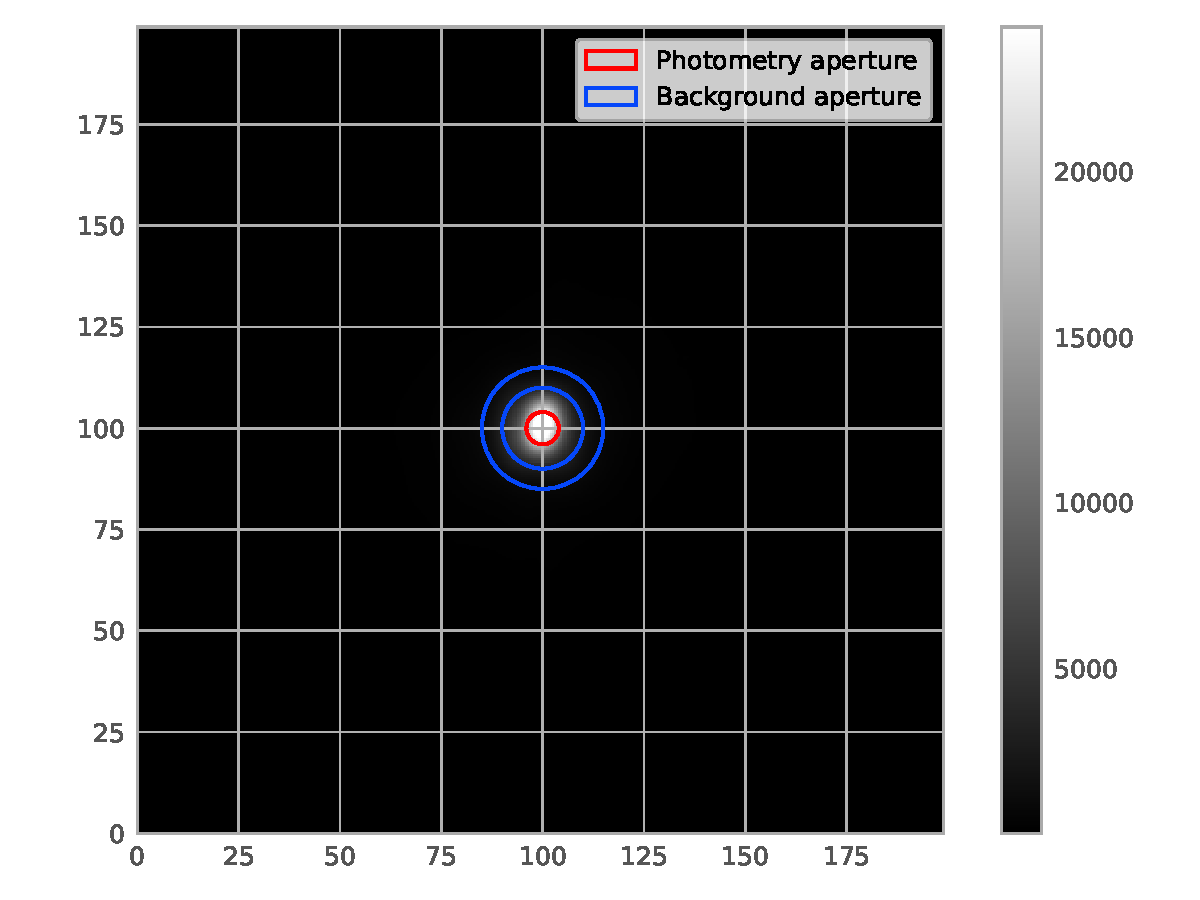
\includegraphics[width=0.9\textwidth]{pics/aperture_example.pdf}
		\caption{An aperture photometry for the star in the center, where the red circle indicates the aperture used and the two blue circles define the annulus used for the background subtraction.}
		\label{fig:aperture_ex}
\end{figure}
From the figure you can see that we chose the annulus not directly after the aperture, but this is just one way to do it. One could also choose the annulus directly after the aperture or choose a different distance between the annulus and the aperture. However the annulus should give a good approximation for the background inside the aperture and therefore it should not be too far away from the aperture. We chose a small distance between the aperture and the annulus of 4 pixels, because we wanted that as little starlight (in this case) as possible is included in the annulus. If we plot the counts per pixels which are inlcuded in a certain radius around the star, as it is done in figure \ref{fig:annulus_radi} we see that after around 10 pixels the increase is decreasing rapidly. That is where there is only little starlight left. This is also why we choose the annulus to go from a radius of 10 to 15 pixels. 
\begin{figure}[H]
	\centering
		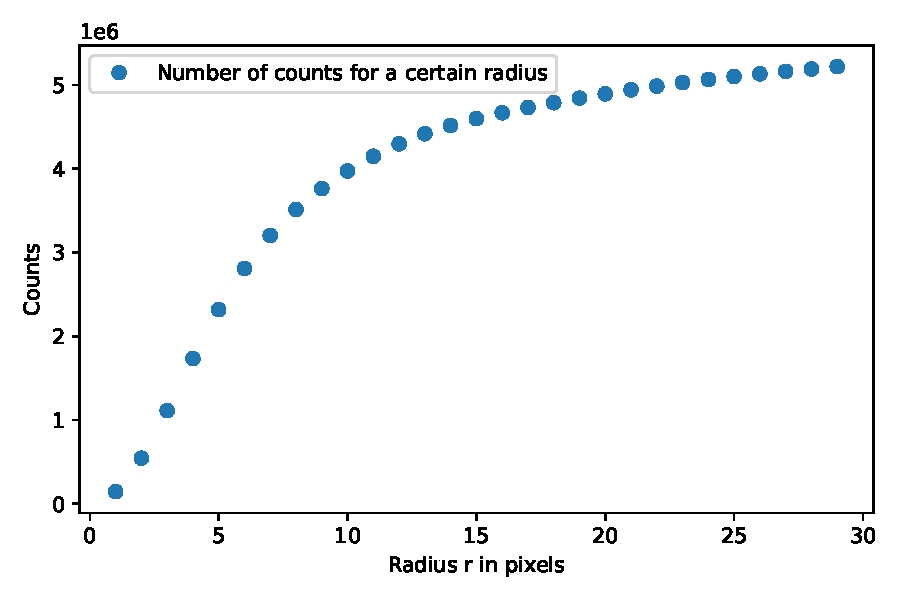
\includegraphics[width=0.8\textwidth]{pics/CountsPerRadius.pdf}
		\caption{The total flux of the star is calculated for different radi and plotted. This shows that after a radius of 10 pixels the contribution from the star is almost gone.}
		\label{fig:annulus_radi}
\end{figure}
Additionally we chose the radius of the aperture to be 6 pixels.

\subsection{Aperture photometry and ghosts}

